
\documentclass{acm_proc_article-sp}

\usepackage{amsmath}
\usepackage{verbatim}
\usepackage{textcomp}
\usepackage{graphicx}
\usepackage{subcaption}
\usepackage{url}
\usepackage{multicol}
\usepackage{tikz}
\usetikzlibrary{positioning}
\usepackage{wasysym}

\tikzset{%
  every neuron/.style={
    circle,
    draw,
    minimum size=1cm
  },
  neuron missing/.style={
    draw=none, 
    scale=3,
    text height=0.333cm,
    execute at begin node=\color{black}$\vdots$
  },
  every filter/.style={
    rectangle,
    draw,
    minimum size=0.5cm
  },
  filter missing/.style={
    draw=none,
    scale=3,
    text height=0.333cm,
    execute at begin node=\color{black}$\vdots$
  },
}

\begin{document}

\title{Difficult Handwritten Digit Classification \\
{\normalsize Code available at: \url{https://github.com/slflmm/Miniproject-3}}} 
\subtitle{COMP 598 -- Miniproject 3 -- Team X}

\numberofauthors{3} 
\author{
% 1st. author
\alignauthor 
Narges Aghakazemjourabbaf\\
	\affaddr{260460855}
\alignauthor
Stephanie Laflamme\\
	\affaddr{260376691}
% 2nd. author
\alignauthor Benjamin La Schiazza\\
	\affaddr{260531181}
% 3rd. author
}

\date{Oct15}



\maketitle
\begin{abstract}

\end{abstract}

\section{Introduction}% overview of approach
- Talk about the dataset and the difficulty with it

- Discuss features

- Discuss learners

\section{Preprocessing}
The raw pixels are standardized. For each example $i$ in the training set, and each feature $j$, we replace it with its standardized value $$x'_{ij} = \cfrac{x_{ij} - \mu_{j}}{\sigma_{j}}.$$

These values for $\mu_j$ and $\sigma_j$ are used to apply the same transformation to the test set examples.

\section{Feature Design and Selection}
When appropriate for the learner, we consider three feature sets; raw pixels, PCA, and Gabor filter-based features. For the open method, we consider contrast-normalized pixels, and add rotation-perturbed examples.

\subsection{Pixels}
We use the post-standardization pixel information as a baseline feature set.This produces feature vectors of length 2304. 

\subsection{PCA}
Principal component analysis (PCA), developed by Pearson in the early 1900s\cite{Pearson}, converts a set of possibly correlated features into a linearly uncorrelated representation, with the resulting features ordered by variance. 

We use the implementation of PCA provided by the Scikit-learn library\cite{scikit-learn}, which uses singular value decomposition of the input data matrix.

As removing the least useful features made the results of our baseline classifier worse, we keep full dimensionality. However, we expect PCA features to produce better results given that they are linearly uncorrelated.

\subsection{Gabor}
Gabor filters are linear filters used for edge detection and are thought to be similar to the early stages of visual processing in humans. Indeed, their frequency and orientations correspond roughly to simple cells in the visual cortex of humans and other mammals; these cells can be modelled with Gabor functions.\cite{Jones}\cite{Marvcelja} As these filters are well-suited to image processing, we attempt to translate them into features.

Previous research has used the energy of the convolution between a Gabor filters and image (a measure of how strongly the filter responds to that image\cite{Grigorescu}) as a feature by summing its magnitudes in the image.\cite{Bau} This is equivalent to using the Frobenius norm of the convolved image as a feature. 

Using the Scikit-learn library\cite{scikit-learn}, we generate 16 Gabor filters with 4 equidistant $\theta$ values, $\sigma = \{1, 3\}$, and frequencies $= \{0.05, 0.25\}$. Figure \ref{fig:gabor} illustrates the effects of $\theta$, $\sigma$, and frequency with a sample of our filters. We form the feature vector of an image in the dataset by collecting the Frobenius norms of the image convolved with each filter. 

\begin{figure}[h]
	\centering
	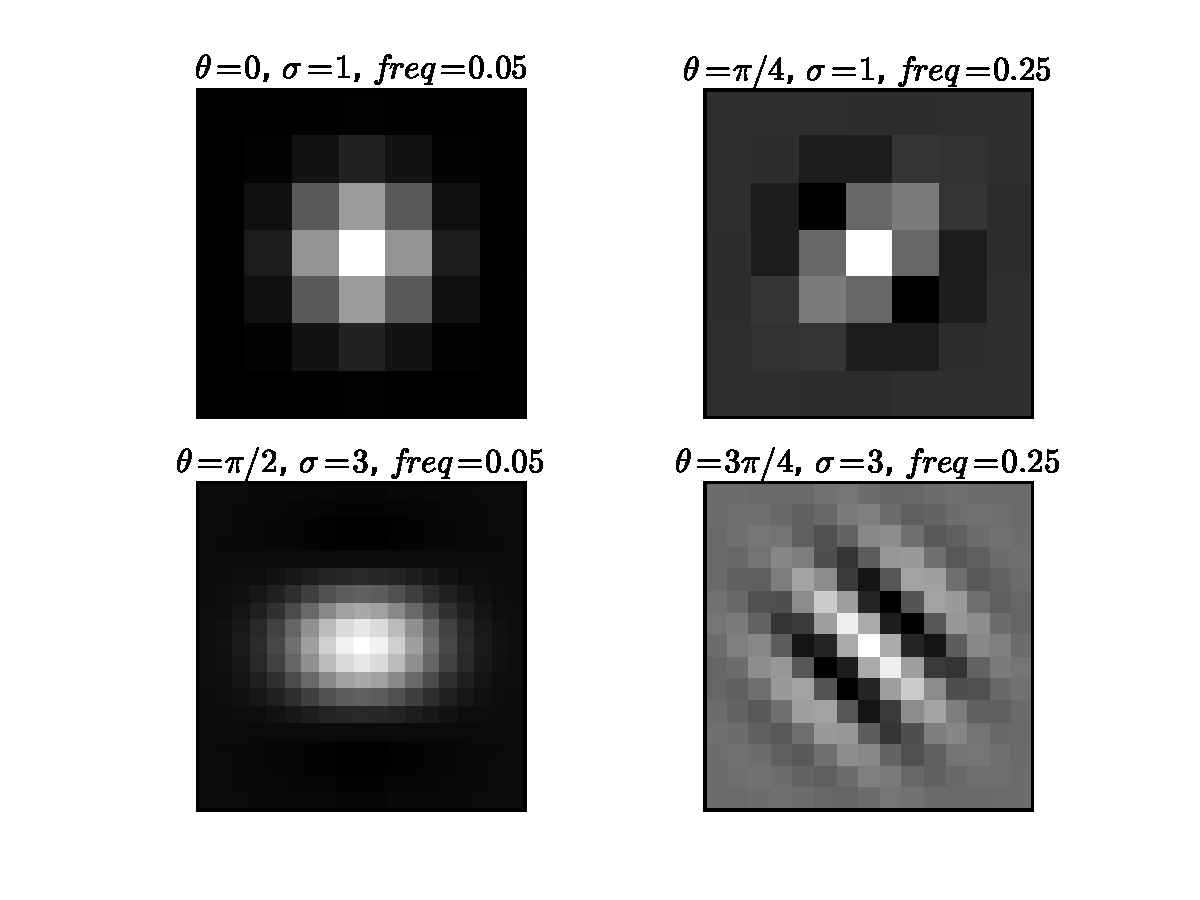
\includegraphics[width=\linewidth]{gabors}
  	\caption{Some Gabor filters}
  	\label{fig:gabor}
\end{figure}

\subsection{Perturbed}


\section{Algorithm Selection}% for each category
\subsection{Perceptron}
We implement a multiclass perceptron as a baseline classifier. Given $n$ examples with $m$ features each, and given $k$ classes, the perceptron learns a matrix $W$ of $m \times k$ weights (one for each feature-class combination) by gradient descent on the error $$Err(x) = (y - f(W^Tx)),$$
where $f$ is the Heaviside step function.

\subsection{Fully-Connected Neural Network}

\subsection{Linear SVM}
Use Scikit-learn implementation \cite{scikit-learn}

\subsection{Convolutional Neural Network}
Although fully-connected neural networks tend to perform very well at machine learning tasks, their ability to classify images can be very affected by shifts in position or shape distortions--in other words, they can be bad at identifying invariant patterns. In the early '80s, Fukushima introduced convolution layers to remedy that problem and handle geometrical similarities regardless of position.\cite{Fukushima} In effect, a convolution acts as a filter applied to an image's raw pixels; a convolution layer contains many such filters, whose weights are learned as the neural network is trained. This serves as an implicit, learned feature extraction at the start of the neural network, typically followed by hidden layers.

The use of convolution layers seem particularly appropriate given the difficulty of our dataset, which adds noise-inducing modifications to the MNIST dataset. Indeed, LeCun has shown that a convolutional neural network trained with MNIST images continues to predict digits correctly regardless of rotations and noise.\cite{LeCun}

It should be noted, however, that neural networks with many layers tend to overfit; there may be many complicated relationships between examples and their labels, and enough hidden units to model these relationships in multiple ways. Hinton et al. introduced the concept of dropout. During training, hidden units are randomly omitted with probability $p$, which helps prevent complex co-adaptations on training data. The combination of dropout with L2 normalization on a neural network trained with minibatch SGD gave Hinton et al. better results than without dropout.\cite{Hinton}  

This idea has been successfully applied to a convolutional neural network; using a network with convolution layers followed by hidden layers, Krizhevsky et al. applied dropout to the hidden layer weights, and vastly outperformed other methods on an ImageNet classification competition.\cite{Krizhevsky} 

In light of these findings, we implement our own convolutional neural network. Its architecture consists of a variable number of convolution layers, followed by a variable number of hidden layers and the output layer. We apply dropout to the hidden layers, and train our network using minibatch SGD, with L2 regularization.

\section{Optimization} % if required
Given the vast amount of time required to train a convolutional neural network, we implement ours to run on a GPU, which allows us to increase the speed of training by approximately factor of 10. We make use of Theano\cite{Theano}, a symbolic Python library that enables compiling computation-heavy functions in C and running them on a GPU.

\section{Parameter Selection Method}% model order, learning rate, etc
For each learner, we fix the hyperparameters to compare the performance of appropriate feature sets, and perform a preliminary manual inspection to identify viable hyperparameters, followed up by either the traditional gridsearch, or a random search. In cases where there are many hyperparameters and training is long, random search offers a faster alternative to gridsearch for finding good hyperparameters. It has been shown to obtain results as good as or better than gridsearch\cite{Bergstra}. The details of parameter selection are discussed in this section.

\subsection{Perceptron}
The perceptron can use pixel, PCA, or Gabor features. We initially fix the hyperparameters to identify the most promising feature set using 5-fold cross-validation. We then consider its two hyperparameters--learning rate and number of learning iterations--and perform gridsearch for $\alpha \in [10^{-4},10^{-1}]$ and the number of iterations ranging form 10 to 35; the averaged validation accuracy from 5-fold cross-validation is used as a measure of success for the hyperparameter setting. 

\subsection{Fully-Connected Neural Network}
The neural network can also use pixel, PCA, or Gabor features. As we did for the perceptron, we fix what appear to be reasonable hyperparameters and identify the best feature set for this classifier using results from 5-fold cross-validation. Then, we perform random search for 15 hyperparameter settings selected over the space of hyperparameters; we use mean accuracy from 5-fold cross-validation to determine the most promising parameter setting. Table \ref{tab:nn-hyp} lists the hyperparameters and the range of values we consider.
\begin{table}[h!]
  \centering
  \begin{tabular}{|l|l|}
    \hline 
    {\bfseries Hyperparameter} & {\bfseries Values}\\
    \hline \hline
    Number of layers & \{1, 2\} \\
    Hidden units per layer & \{10, 15, ..., 50\} \\
    Learning rate & $(0, 0.1]$ \\
    Momentum & $[0.1, 0.9]$ \\
    Training epochs & $\{50, ..., 200\}$ \\
    \hline
  \end{tabular}
  \caption{Neural network hyperparameters and their considered values}
  \label{tab:nn-hyp}
\end{table}


\subsection{Linear SVM}

\subsection{Convolutional Neural Network}
The only appropriate features for a convolutional neural network are pixel features. In this case, rather than using per-feature standardization, we apply contrast normalization within images.

We must optimize many hyperparameters; in addition to those for the fully-connected neural network, we must also consider the dropout rate, as well as the number of convolution layers, the number of filters per layer, and the filter sizes. Due to time constraints, we can only sample a small portion of this very large parameter space. Hence, we select hyperparameters with manual search.

Luckily, we can use heuristics to reduce our search space when it comes to the size of hidden layers and the size and number of filters per convolution layer. To start with, tips and tricks offered by Theano's deep learning tutorials note that, to preserve information across convolution layers, the value of (number of feature maps $\times$ number of incoming pixels) is usually chosen to be constant. Moreover, it is suggested that $5 \times 5$ filters in the first convolution layer work well with the MNIST dataset, while filter sizes of $12\times12$ or $15\times15$ work well with images with hundreds of pixels in each dimension.\cite{Theano-tut} Noting that MNIST images are $28\times28$ pixels, whereas our dataset's images are $48\times48$ pixels, we consider filter sizes ranging from $5\times 5$ to $8\times 8$. We begin with 3 convolution layers, with 20 to 50 filters per layer; we adjust the number of filters of later layers as a function of the values for the first layer.

We use one hidden layer; as discussed in class, with binary inputs, the number of hidden units in a hidden layer should be around $\log(n\_inputs)$, where $n\_inputs$ is the number of connections going into the layer. Since our inputs are not binary, we start with $10\times \log(n\_inputs)$ hidden units.

\section{Testing and Validation}%detailed analysis of results

\subsection{Perceptron}
In a primary step, we performed 5-fold cross-validation to compare raw pixels, PCA, and Gabor features using a fixed learning rate ($\alpha = 0.01$) and number of iterations (15). As shown in Table \ref{tab:perc-features}, PCA features were the most performant, with a validation accuracy of 26.282\%.
\begin{table}[h!]
  \centering
  \begin{tabular}{|c||c|c|c| }
    \hline
    {\bfseries Features} & Pixels & PCA & Gabor \\
    \hline
    {\bfseries Accuracy} & 25.794 & 26.282 & 10.398 \\
    \hline
  \end{tabular}
  \caption{Mean validation accuracy of perceptron using different features}
  \label{tab:perc-features}
\end{table}

Using PCA features, we performed 5-fold cross-validation over the learning rate $\alpha$ and the number of training iterations of the perceptron model. Figure \ref{fig:perc-gridsearch} shows the results of gridsearch with both parameters. The precise values of the best parameters found by the gridsearch cross-validation procedure were $\alpha = 0.0005$ with 25 training iterations, yielding a mean validation accuracy of 26.598\%.\footnote{Additional results showing training error vs validation error are shown in Appendix \ref{sec:additional-results}}
\begin{figure}[h!]
	\centering
	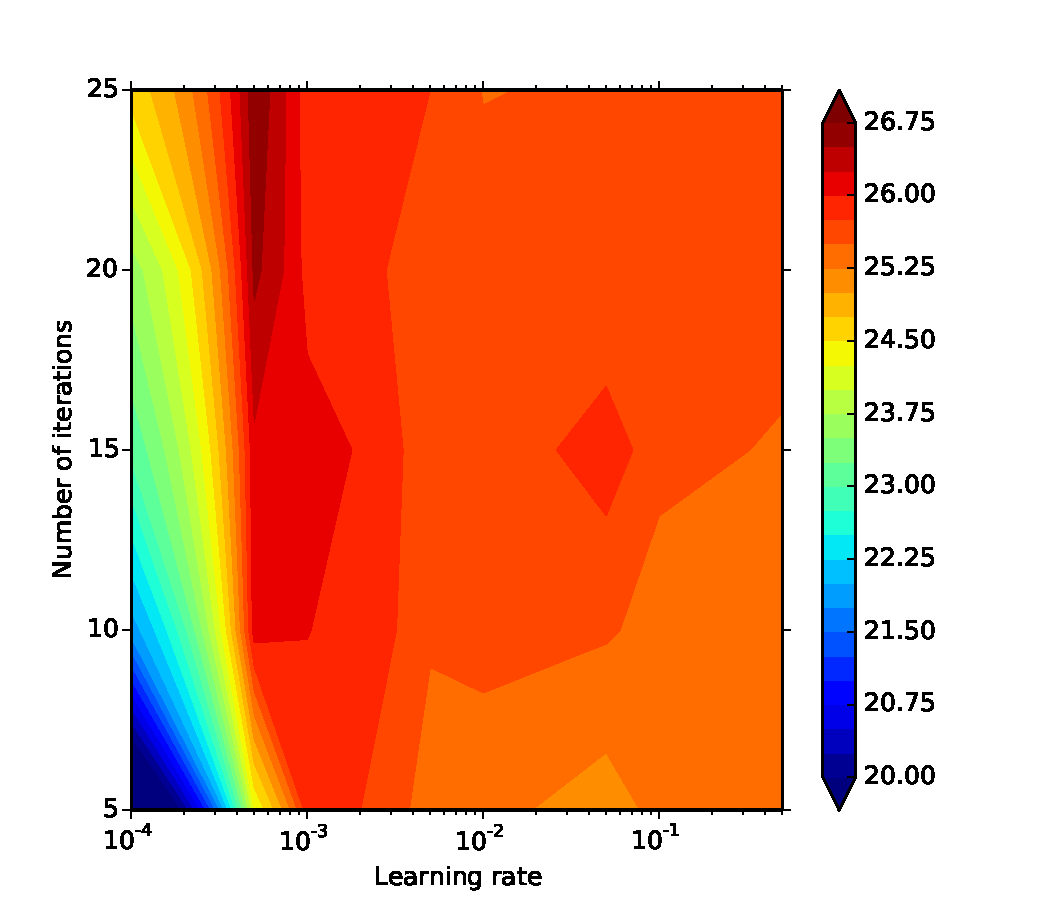
\includegraphics[width=\linewidth]{perceptron_gridsearch}
  	\caption{Mean cross-validation accuracy as a function of parameters $\alpha$ and number of iterations}
  	\label{fig:perc-gridsearch}
\end{figure}

After training our perceptron on the complete training set using these parameters, we submitted our results to Kaggle and obtained a test accuracy of 27.420\%. As an approximation of the test confusion matrix, we provide the confusion matrix for the combined validation sets in Figure \ref{fig:perc-confusion}. Note the perceptron's greater ability to identify 0s and 1s compared to other digits.
\begin{figure}[h!]
	\centering
	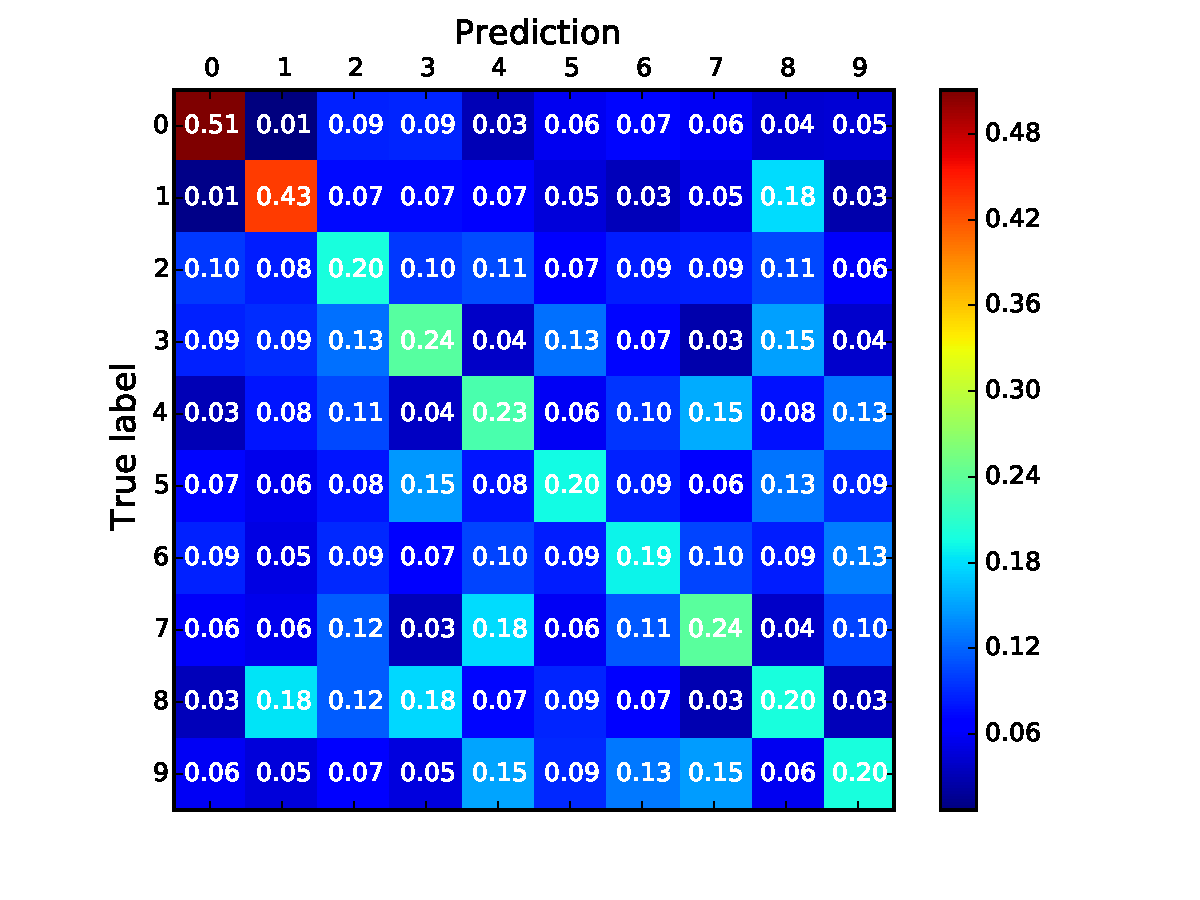
\includegraphics[width=\linewidth]{perceptron_confusion}
  	\caption{Validation confusion matrix for perceptron}
  	\label{fig:perc-confusion}
\end{figure}

\subsection{Fully-Connected Neural Network}
Try a baseline net with the three feature sets, compare (5-fold cross-validation).

Use the best feature set to find best hyperparameters with cross-validation. You should probably try random search rather than gridsearch (faster and just as good or better), for some set number of configurations. Use some graph to show the hyperparameter space results. Plot validation confusion matrix. Say the test set (kaggle) result using best model found during crossval.

\subsection{Linear SVM}

\subsection{Convolutional Neural Network}


SHOW THE FINAL NETWORK ARCHITECTURE Figure \ref{fig:convnet-architect}

(something like this, but the architecture is totally subject to change)
\begin{figure}[h!]
\centering
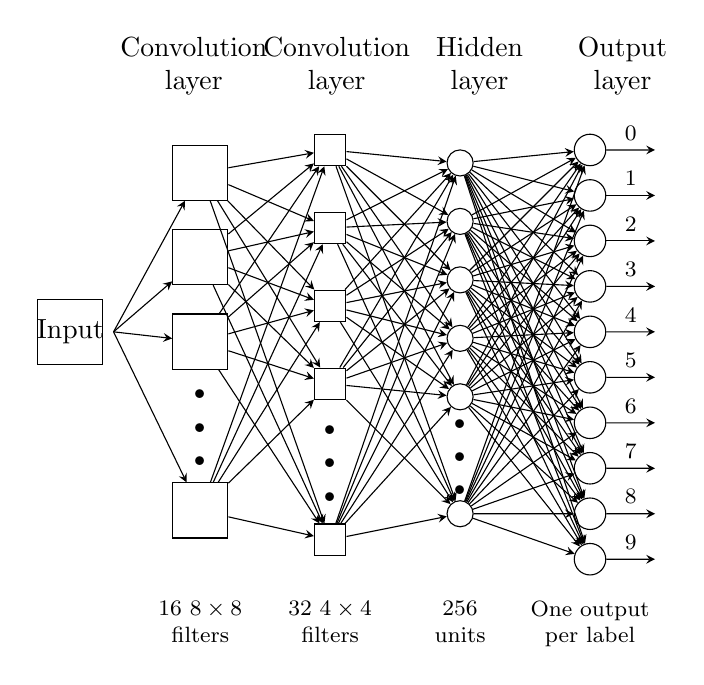
\begin{tikzpicture}[x=1.5cm, y=1.5cm, >=stealth, scale=0.55]

\draw[fill=white] (-0.5,-2) rectangle (0.5,-1); \node (input) at (0,-1.5) {Input};

% Input conv layer
\foreach \m/\l [count=\y] in {1,2,3,missing,4}
  \node [every filter/.try, filter \m/.try, minimum size=0.70cm] (conv1-\m) at (2,2.25-\y*1.3) {};

% Second conv layer
\foreach \m [count=\y] in {1,2,3,4,missing,5}
  \node [every filter/.try, filter \m/.try, minimum size=0.40cm ] (conv2-\m) at (4,2.5-\y*1.2) {};

% Hidden layer
\foreach \m [count=\y] in {1,2,3,4,5,missing,6}
  \node [every neuron/.try, neuron \m/.try, minimum size=0.25cm] (hidden-\m) at (6,2-\y*0.9) {};

% Output layer
\foreach \m [count=\y] in {0,1,2,3,4,5,6,7,8,9}
  \node [every neuron/.try, neuron\m/.try, minimum size=0.4cm] (output-\m) at (8, 2.0-\y*0.7){};

% ALL OF THE ARROWS
\foreach \i in {1, ..., 4}
  \draw [->] (input.east) -- (conv1-\i);

\foreach \i in {1, ..., 4}
  \foreach \j in {1,...,5}
    \draw [->] (conv1-\i) -- (conv2-\j);

\foreach \i in {1, ..., 5}
  \foreach \j in {1,...,6}
    \draw [->] (conv2-\i) -- (hidden-\j);

\foreach \i in {1,...,6}
  \foreach \j in {0,...,9}
    \draw [->] (hidden-\i) -- (output-\j);


% Node names for output
\foreach \I in {0,...,9}
 \draw [->] (output-\I) -- ++(1,0)
  node [above, midway, font=\footnotesize] {$\I$};


\foreach \l [count=\x from 0] in {Convolution, Convolution, Hidden, Output}
  \node [align=center, above] at (1.9 + \x*2.2,2) {\l \\ layer};

\foreach \l [count=\x from 0] in {16 $8\times8$\\ filters, 32 $4\times4$\\ filters, 256\\ units, One output\\ per label}
  \node [align=center, below, font=\footnotesize] at (2 + \x*2,-5.5) {\l};


\end{tikzpicture}
\caption{Convolutional neural network final architecture}
\label{fig:convnet-architect}
\end{figure}


\section{Discussion}% pros/cons of approach & methodology (and alternatives)
Why is it better at classifying 0s and 1s? (Check number of examples in classes--could be Benford's law?

Using Gabor filters as a kernel rather than feature \cite{Sabri}

Other version of dropout \cite{Wan}

Pretraining \cite{Erhan}

Others: \cite{Rowley}, \cite{Simard}

{\bfseries We hereby state that all the work presented in this report is that of the authors.}

\bibliographystyle{abbrv}
\bibliography{references}

\appendix
\label{appendix}

\section{Additional results}
\label{sec:additional-results}

\begin{figure}[h!]
	\centering
	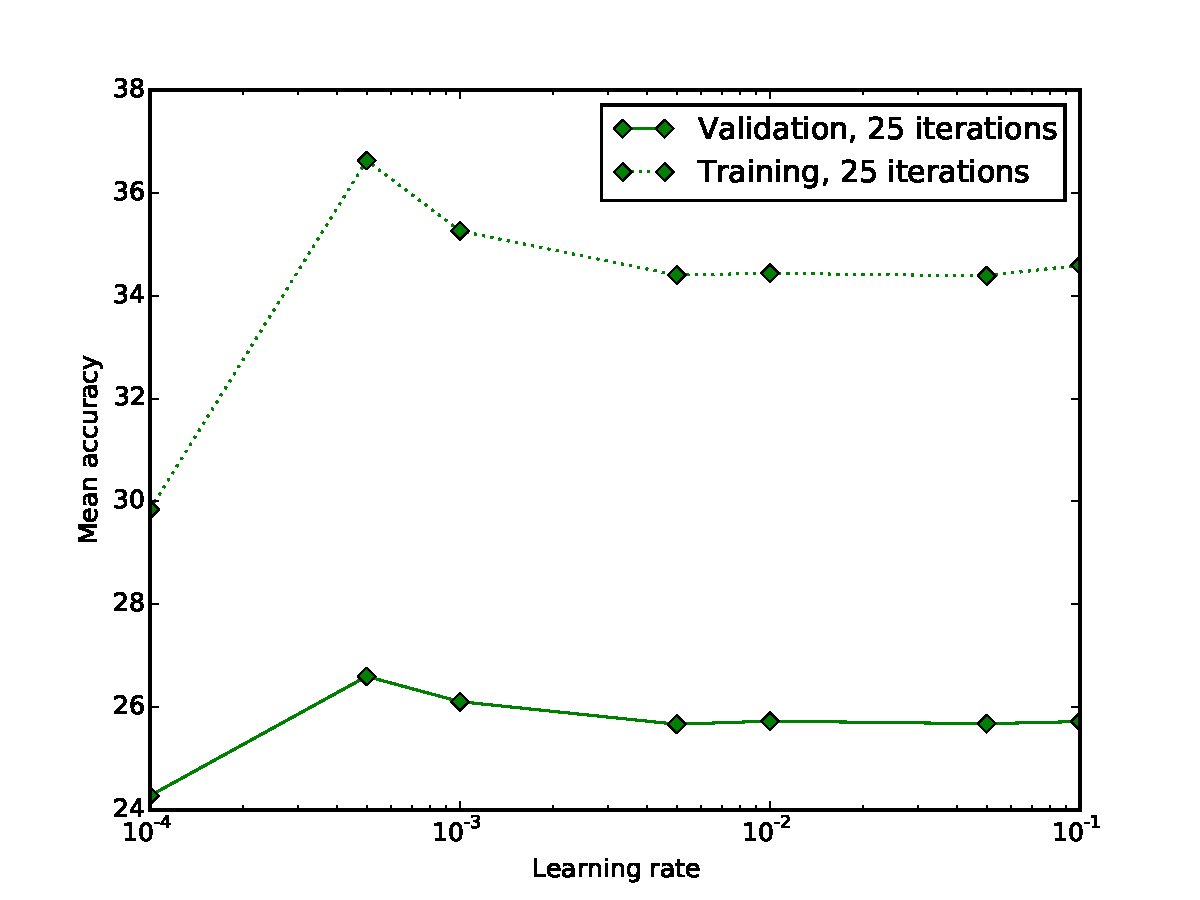
\includegraphics[width=\linewidth]{perceptron_learningrate}
  	\caption{Cross-validation over $\alpha$ with perceptron, keeping \# iterations optimal}
  	\label{fig:perc-learningrate}
\end{figure}
\begin{figure}[h!]
	\centering
	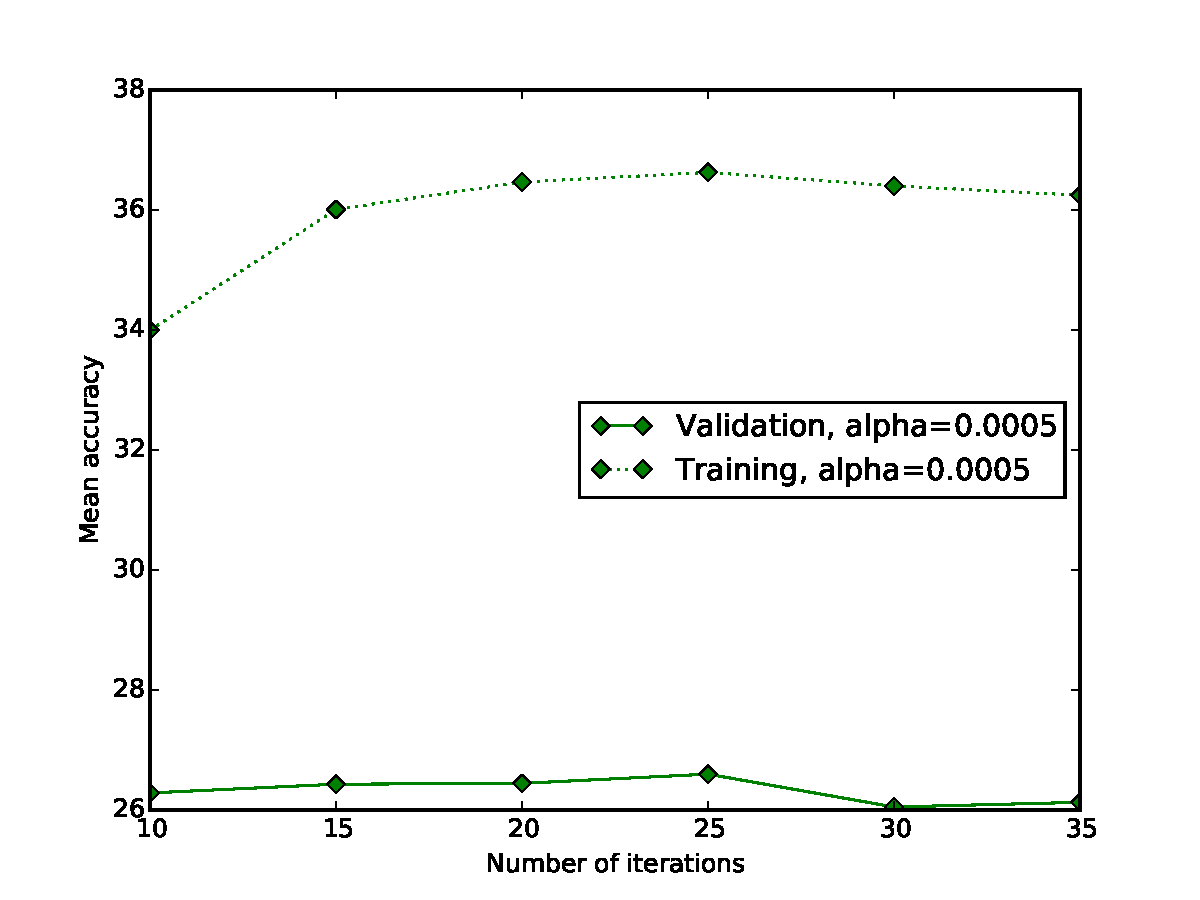
\includegraphics[width=\linewidth]{perceptron_iterations}
  	\caption{Cross-validation over \# of iterations with perceptron, keeping $\alpha$ optimal}
  	\label{fig:perc-iterations}
\end{figure}


\balancecolumns
\end{document}